\usetikzlibrary{calc}
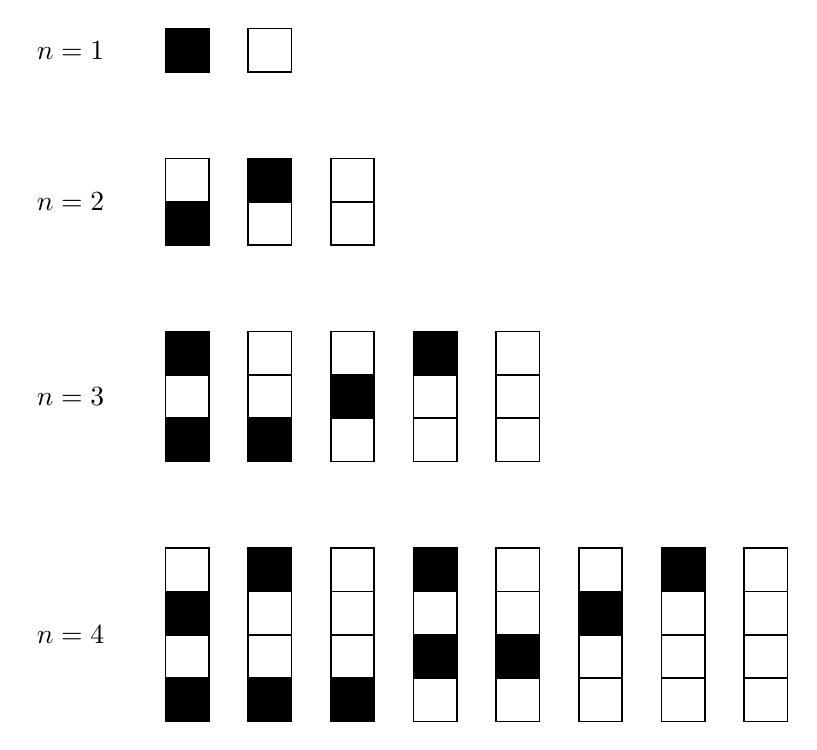
\begin{tikzpicture}[x=1cm,y=1cm,line width=.6pt,font=\normalsize]
% Row n=1: 2 columns x 1 cell
\node[anchor=east] at (1.55,8.525) {$n=1$};
% CELL n=1 c=1 r=1 color=B
\filldraw[fill=black,draw=black] (2.2,8.25) rectangle (2.75,8.8);
% CELL n=1 c=2 r=1 color=W
\draw[draw=black] (3.25,8.25) rectangle (3.8,8.8);
% Row n=2: 3 columns x 2 cells
\node[anchor=east] at (1.55,6.6) {$n=2$};
% CELL n=2 c=1 r=1 color=W
\draw[draw=black] (2.2,6.6) rectangle (2.75,7.15);
% CELL n=2 c=1 r=2 color=B
\filldraw[fill=black,draw=black] (2.2,6.05) rectangle (2.75,6.6);
% CELL n=2 c=2 r=1 color=B
\filldraw[fill=black,draw=black] (3.25,6.6) rectangle (3.8,7.15);
% CELL n=2 c=2 r=2 color=W
\draw[draw=black] (3.25,6.05) rectangle (3.8,6.6);
% CELL n=2 c=3 r=1 color=W
\draw[draw=black] (4.3,6.6) rectangle (4.85,7.15);
% CELL n=2 c=3 r=2 color=W
\draw[draw=black] (4.3,6.05) rectangle (4.85,6.6);
% Row n=3: 5 columns x 3 cells
\node[anchor=east] at (1.55,4.125) {$n=3$};
% CELL n=3 c=1 r=1 color=B
\filldraw[fill=black,draw=black] (2.2,4.4) rectangle (2.75,4.95);
% CELL n=3 c=1 r=2 color=W
\draw[draw=black] (2.2,3.85) rectangle (2.75,4.4);
% CELL n=3 c=1 r=3 color=B
\filldraw[fill=black,draw=black] (2.2,3.3) rectangle (2.75,3.85);
% CELL n=3 c=2 r=1 color=W
\draw[draw=black] (3.25,4.4) rectangle (3.8,4.95);
% CELL n=3 c=2 r=2 color=W
\draw[draw=black] (3.25,3.85) rectangle (3.8,4.4);
% CELL n=3 c=2 r=3 color=B
\filldraw[fill=black,draw=black] (3.25,3.3) rectangle (3.8,3.85);
% CELL n=3 c=3 r=1 color=W
\draw[draw=black] (4.3,4.4) rectangle (4.85,4.95);
% CELL n=3 c=3 r=2 color=B
\filldraw[fill=black,draw=black] (4.3,3.85) rectangle (4.85,4.4);
% CELL n=3 c=3 r=3 color=W
\draw[draw=black] (4.3,3.3) rectangle (4.85,3.85);
% CELL n=3 c=4 r=1 color=B
\filldraw[fill=black,draw=black] (5.35,4.4) rectangle (5.9,4.95);
% CELL n=3 c=4 r=2 color=W
\draw[draw=black] (5.35,3.85) rectangle (5.9,4.4);
% CELL n=3 c=4 r=3 color=W
\draw[draw=black] (5.35,3.3) rectangle (5.9,3.85);
% CELL n=3 c=5 r=1 color=W
\draw[draw=black] (6.4,4.4) rectangle (6.95,4.95);
% CELL n=3 c=5 r=2 color=W
\draw[draw=black] (6.4,3.85) rectangle (6.95,4.4);
% CELL n=3 c=5 r=3 color=W
\draw[draw=black] (6.4,3.3) rectangle (6.95,3.85);
% Row n=4: 8 columns x 4 cells
\node[anchor=east] at (1.55,1.1) {$n=4$};
% CELL n=4 c=1 r=1 color=W
\draw[draw=black] (2.2,1.65) rectangle (2.75,2.2);
% CELL n=4 c=1 r=2 color=B
\filldraw[fill=black,draw=black] (2.2,1.1) rectangle (2.75,1.65);
% CELL n=4 c=1 r=3 color=W
\draw[draw=black] (2.2,0.55) rectangle (2.75,1.1);
% CELL n=4 c=1 r=4 color=B
\filldraw[fill=black,draw=black] (2.2,0.0) rectangle (2.75,0.55);
% CELL n=4 c=2 r=1 color=B
\filldraw[fill=black,draw=black] (3.25,1.65) rectangle (3.8,2.2);
% CELL n=4 c=2 r=2 color=W
\draw[draw=black] (3.25,1.1) rectangle (3.8,1.65);
% CELL n=4 c=2 r=3 color=W
\draw[draw=black] (3.25,0.55) rectangle (3.8,1.1);
% CELL n=4 c=2 r=4 color=B
\filldraw[fill=black,draw=black] (3.25,0.0) rectangle (3.8,0.55);
% CELL n=4 c=3 r=1 color=W
\draw[draw=black] (4.3,1.65) rectangle (4.85,2.2);
% CELL n=4 c=3 r=2 color=W
\draw[draw=black] (4.3,1.1) rectangle (4.85,1.65);
% CELL n=4 c=3 r=3 color=W
\draw[draw=black] (4.3,0.55) rectangle (4.85,1.1);
% CELL n=4 c=3 r=4 color=B
\filldraw[fill=black,draw=black] (4.3,0.0) rectangle (4.85,0.55);
% CELL n=4 c=4 r=1 color=B
\filldraw[fill=black,draw=black] (5.35,1.65) rectangle (5.9,2.2);
% CELL n=4 c=4 r=2 color=W
\draw[draw=black] (5.35,1.1) rectangle (5.9,1.65);
% CELL n=4 c=4 r=3 color=B
\filldraw[fill=black,draw=black] (5.35,0.55) rectangle (5.9,1.1);
% CELL n=4 c=4 r=4 color=W
\draw[draw=black] (5.35,0.0) rectangle (5.9,0.55);
% CELL n=4 c=5 r=1 color=W
\draw[draw=black] (6.4,1.65) rectangle (6.95,2.2);
% CELL n=4 c=5 r=2 color=W
\draw[draw=black] (6.4,1.1) rectangle (6.95,1.65);
% CELL n=4 c=5 r=3 color=B
\filldraw[fill=black,draw=black] (6.4,0.55) rectangle (6.95,1.1);
% CELL n=4 c=5 r=4 color=W
\draw[draw=black] (6.4,0.0) rectangle (6.95,0.55);
% CELL n=4 c=6 r=1 color=W
\draw[draw=black] (7.45,1.65) rectangle (8.0,2.2);
% CELL n=4 c=6 r=2 color=B
\filldraw[fill=black,draw=black] (7.45,1.1) rectangle (8.0,1.65);
% CELL n=4 c=6 r=3 color=W
\draw[draw=black] (7.45,0.55) rectangle (8.0,1.1);
% CELL n=4 c=6 r=4 color=W
\draw[draw=black] (7.45,0.0) rectangle (8.0,0.55);
% CELL n=4 c=7 r=1 color=B
\filldraw[fill=black,draw=black] (8.5,1.65) rectangle (9.05,2.2);
% CELL n=4 c=7 r=2 color=W
\draw[draw=black] (8.5,1.1) rectangle (9.05,1.65);
% CELL n=4 c=7 r=3 color=W
\draw[draw=black] (8.5,0.55) rectangle (9.05,1.1);
% CELL n=4 c=7 r=4 color=W
\draw[draw=black] (8.5,0.0) rectangle (9.05,0.55);
% CELL n=4 c=8 r=1 color=W
\draw[draw=black] (9.55,1.65) rectangle (10.1,2.2);
% CELL n=4 c=8 r=2 color=W
\draw[draw=black] (9.55,1.1) rectangle (10.1,1.65);
% CELL n=4 c=8 r=3 color=W
\draw[draw=black] (9.55,0.55) rectangle (10.1,1.1);
% CELL n=4 c=8 r=4 color=W
\draw[draw=black] (9.55,0.0) rectangle (10.1,0.55);
\end{tikzpicture}
